\documentclass[12pt, oneside, titlepage]{article}   	% use "amsart" instead of "article" for AMSLaTeX format

\usepackage{graphicx}
\graphicspath{ {\string} }
\usepackage{subcaption}

%%%%%%%%%%%%%%%%%%%%%%%%%%%%%%%%%%%%%%%%%%%%%%%%%%%%
% set up packages
%%%%%%%%%%%%%%%%%%%%%%%%%%%%%%%%%%%%%%%%%%%%%%%%%%%%
\usepackage{geometry}                
\usepackage{textcomp}                
\usepackage{amsmath}                
\usepackage{graphicx}                
\usepackage{amssymb}                
\usepackage{fancyhdr}                
\usepackage{subcaption}                
\usepackage{bm}                
\usepackage{lineno}
% package for comments
\usepackage{soul}

\usepackage[breaklinks=true]{hyperref}

\usepackage[superscript,noadjust]{cite} % puts dash in citations to abbreviate
\usepackage [autostyle, english = american]{csquotes} % sets US-style quotes

\usepackage{etoolbox} % block quotes

\usepackage{float}
\usepackage{color}

\usepackage{pgf}
\usepackage{tikz}
\usepackage{eqnarray}

\usepackage{listings} % code blocks
\usepackage{setspace}

\usepackage{lscape}

% tikz background
\usetikzlibrary{backgrounds, fit}


\usepackage{natbib}
%\bibliographystyle{abbrvnat}
\setcitestyle{authoryear,open={(},close={)}}

%%%%%%%%%%%%%%%%%%%%%%%%%%%%%%%%%%%%%%%%%%%%%%%%%%%%
% call packages
%%%%%%%%%%%%%%%%%%%%%%%%%%%%%%%%%%%%%%%%%%%%%%%%%%%%	
\geometry{letterpaper, marginparwidth=60pt} % sets up geometry              		
\linenumbers % adds line numbers 
\MakeOuterQuote{"} % sets quote style
\doublespacing % setspace

%%%%%%%%%%%%%%%%%%%%%%%%%%%%%%%%%%%%%%%%%%%%%%%%%%%%
% patches with etoolbox 
%%%%%%%%%%%%%%%%%%%%%%%%%%%%%%%%%%%%%%%%%%%%%%%%%%%%	
% block quotes
\AtBeginEnvironment{quote}{\small}

% linenumbers
\makeatletter
\patchcmd{\@startsection}{\@ifstar}{\nolinenumbers\@ifstar}{}{}
\patchcmd{\@xsect}{\ignorespaces}{\linenumbers\ignorespaces}{}{}
\makeatother

%%%%%%%%%%%%%%%%%%%%%%%%%%%%%%%%%%%%%%%%%%%%%%%%%%%%
% tikzlibrary modifications
%%%%%%%%%%%%%%%%%%%%%%%%%%%%%%%%%%%%%%%%%%%%%%%%%%%%	
\usetikzlibrary{fit}
\usetikzlibrary{positioning}
\usetikzlibrary{arrows}
\usetikzlibrary{automata}

%%%%%%%%%%%%%%%%%%%%%%%%%%%%%%%%%%%%%%%%%%%%%%%%%%%%
% page formatting; exact 1 in margins
%%%%%%%%%%%%%%%%%%%%%%%%%%%%%%%%%%%%%%%%%%%%%%%%%%%%
\pagestyle{plain}                                                     

\setlength{\textwidth}{6.5in}    
\setlength{\oddsidemargin}{0in}
\setlength{\evensidemargin}{0in}
\setlength{\textheight}{8.5in}
\setlength{\topmargin}{0in}
\setlength{\headheight}{0in}
\setlength{\headsep}{0in}
\setlength{\footskip}{.5in}

%%%%%%%%%%%%%%%%%%%%%%%%%%%%%%%%%%%%%%%%%%%%%%%%%%%%
% defining code blocks using listings package
%%%%%%%%%%%%%%%%%%%%%%%%%%%%%%%%%%%%%%%%%%%%%%%%%%%%

\definecolor{dkgreen}{rgb}{0,0.6,0}
\definecolor{gray}{rgb}{0.5,0.5,0.5}
\definecolor{mauve}{rgb}{0.58,0,0.82}

\lstset{frame=tb,
  language=R,
  aboveskip=3mm,
  belowskip=3mm,
  showstringspaces=false,
  columns=flexible,
  basicstyle={\small\ttfamily},
  numbers=none,
  numberstyle=\tiny\color{gray},
 % keywordstyle=\color{blue},
  commentstyle=\color{dkgreen},
  stringstyle=\color{mauve},
  breaklines=true,
  breakatwhitespace=true,
  tabsize=3,
  otherkeywords={0,1,2,3,4,5,6,7,8,9},
  deletekeywords={data,frame,length,as,character,dunif,ps},
}

%%%%%%%%%%%%%%%%%%%%%%%%%%%%%%%%%%%%%%%%%%%%%%%%%%%%
%%%%%%%%%%%%%%%%%%%%%%%%%%%%%%%%%%%%%%%%%%%%%%%%%%%%
% begin document
%%%%%%%%%%%%%%%%%%%%%%%%%%%%%%%%%%%%%%%%%%%%%%%%%%%%
%%%%%%%%%%%%%%%%%%%%%%%%%%%%%%%%%%%%%%%%%%%%%%%%%%%%

\begin{document}

The models below represent the joint likelihood for data from the seed bag experiments. All data from seed bags and viability trials is in the form of binomial trials: we have counts of seeds at the start and end of an experimental window of time. All models for the parameters $\theta_1, \theta_2, \theta_3, \theta_4, \theta_5$ have the same structure for seeds in bag $i$ in year $j$ in population $k$. If the number of seeds starting the trial (trials) is $n_{ijk}$ and the number of seeds at the end of the trial (successes) is $y_{ijk}$, we write a model that has a population-level mean and year-level means drawn from the population-level distribution. The probability of success for each bag is drawn from this year- and population-level distribution:

I compared convergence diagnostics (R-hat, effective sample size) for centered and non-centered parameterizations of the model. Here, I use the centered parameterization because this led to improved convergence. In each model, we obtain the population-level posterior distribution probability of success (the $\theta$s) by marginalizing across years and taking the inverse logit.

\clearpage
\newpage

\subsection*{Seed survival and germination rates for 1-year old seeds}
%%%%%%%%%%%%%%%%%%%%%%%%%%%%%%%%%%%%%%%%%%%%%%%%%%%%
% DIRECTED ACYCLIC GRAPHS FOR AGE 1 SEED BAGS
%%%%%%%%%%%%%%%%%%%%%%%%%%%%%%%%%%%%%%%%%%%%%%%%%%%%
\begin{figure}[h]%
\begin{subfigure}[c]{\textwidth}
\centering
   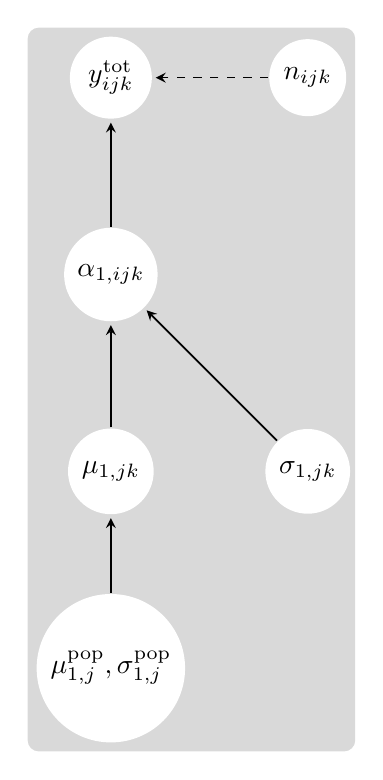
\begin{tikzpicture}[
            > = stealth, % arrow head style
            shorten > = 1pt, % don't touch arrow head to node
            auto,
            node distance = 2.5cm, % distance between nodes
            semithick % line style
        ]

        \tikzstyle{every state}=[
            draw = none,
            thick,
            fill = white,
            minimum size = 4mm
        ]F


	% data level
        \node[state] (Y) [] {$y^{\mathrm{tot}}_{ijk}$};
        \node[state] (N) [right of=Y] {$n_{ijk}$};
       
        \path[dashed,->] (N) edge node {} (Y);

        % probability
        % \node[state] (T) [below of = Y] {$\theta_{ijk}$};
        %       
        % \path[->] (T) edge node {} (Y);
                  
                  % hyperparameters
         \node[state] (AB) [below of = Y] {$\alpha_{1,ijk}$};
                
         \path[->] (AB) edge node {} (Y);
         
          % hyperparameters
        
         \node[state] (MS) [below of = AB] {$\mu_{1,jk}$};
         \node[state] (A) [ right of = MS]  {$\sigma_{1,jk}$};
         
         \path[->] (A) edge node {} (AB);       
         \path[->] (MS) edge node {} (AB);       
         
         \node[state] (H) [below of = MS] {$\mu^\mathrm{pop}_{1,j},\sigma^\mathrm{pop}_{1,j}$};
         \path[->] (H) edge node {} (MS);       

          \begin{scope}[on background layer]
   \node [fit=(Y) (N) (H), fill= gray!30, rounded corners, inner sep=.1cm] {};
  \end{scope}
  
  \end{tikzpicture}
  %
    \hspace{1cm}% NO SPACE!
  % BEGIN FIGURE 3
   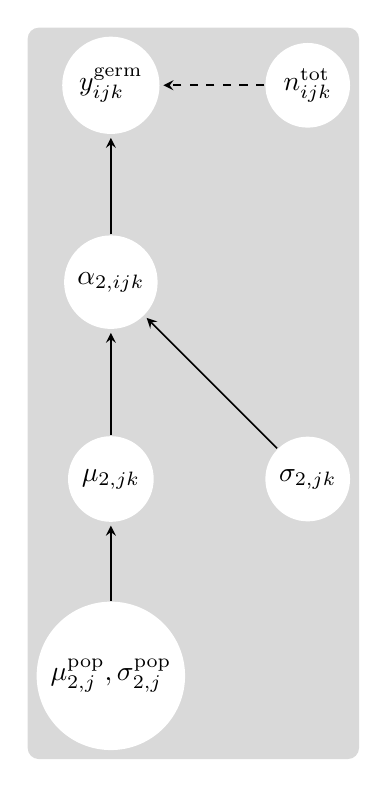
\begin{tikzpicture}[
            > = stealth, % arrow head style
            shorten > = 1pt, % don't touch arrow head to node
            auto,
            node distance = 2.5cm, % distance between nodes
            semithick % line style
        ]

        \tikzstyle{every state}=[
            draw = none,
            thick,
            fill = white,
            minimum size = 4mm
        ]F


	% data level
        \node[state] (Y) [] {$y^{\mathrm{germ}}_{ijk}$};
        \node[state] (N) [right of=Y] {$n^{\mathrm{tot}}_{ijk}$};
       
        \path[dashed,->] (N) edge node {} (Y);

        % probability
        % \node[state] (T) [below of = Y] {$\theta_{ijk}$};
        %       
        % \path[->] (T) edge node {} (Y);
                  
                  % hyperparameters
         \node[state] (AB) [below of = Y] {$\alpha_{2,ijk}$};
                
         \path[->] (AB) edge node {} (Y);
         
          % hyperparameters
        
         \node[state] (MS) [below of = AB] {$\mu_{2,jk}$};
         \node[state] (A)[ right of = MS]  {$\sigma_{2,jk}$};
         
         \path[->] (A) edge node {} (AB);       
         \path[->] (MS) edge node {} (AB);       
         
         \node[state] (H) [below of = MS] {$\mu^\mathrm{pop}_{2,j},\sigma^\mathrm{pop}_{2,j}$};
         \path[->] (H) edge node {} (MS);       
          
                    \begin{scope}[on background layer]
   \node [fit=(Y) (N) (H), fill= gray!30, rounded corners, inner sep=.1cm] {};
  \end{scope}
                 
  \end{tikzpicture}
  %
    \hspace{1cm}% NO SPACE!
  % BEGIN FIGURE 3
   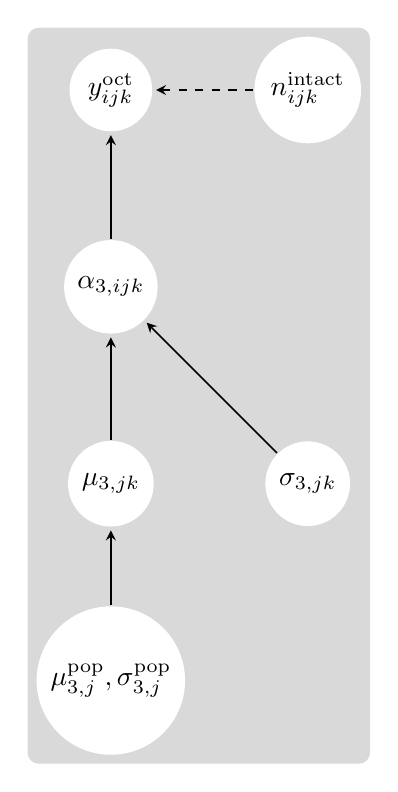
\begin{tikzpicture}[
            > = stealth, % arrow head style
            shorten > = 1pt, % don't touch arrow head to node
            auto,
            node distance = 2.5cm, % distance between nodes
            semithick % line style
        ]

        \tikzstyle{every state}=[
            draw = none,
            thick,
            fill = white,
            minimum size = 4mm
        ]F


	% data level
        \node[state] (Y) [] {$y^{\mathrm{oct}}_{ijk}$};
        \node[state] (N) [right of=Y] {$n^{\mathrm{intact}}_{ijk}$};
       
        \path[dashed,->] (N) edge node {} (Y);

        % probability
        % \node[state] (T) [below of = Y] {$\theta_{ijk}$};
        %       
        % \path[->] (T) edge node {} (Y);
                  
                  % hyperparameters
         \node[state] (AB) [below of = Y] {$\alpha_{3,ijk}$};
                
         \path[->] (AB) edge node {} (Y);
         
          % hyperparameters
        
         \node[state] (MS) [below of = AB] {$\mu_{3,jk}$};
         \node[state] (A) [ right of = MS] {$\sigma_{3,jk}$};
         
         \path[->] (A) edge node {} (AB);       
         \path[->] (MS) edge node {} (AB);       
         
         \node[state] (H) [below of = MS] {$\mu^\mathrm{pop}_{3,j},\sigma^\mathrm{pop}_{3,j}$};
         \path[->] (H) edge node {} (MS);      
         
                   \begin{scope}[on background layer]
   \node [fit=(Y) (N) (H), fill= gray!30, rounded corners, inner sep=.1cm] {};
  \end{scope} 
                 
  \end{tikzpicture}
\subcaption{Directed acyclic graphs for the hierarchical models for seed bag rates. Solid arrows depict the relationships among random variables, and dashed arrows depict the deterministic relationships.}
\end{subfigure}
\end{figure}
%
%%%%%%%%%%%%%%%%%%%%%%%%%%%%%%%%%%%%%%%%%%%%%%%%%%%%
% POSTERIOR AND JOINT DISTRIBUTIONS FOR AGE 1 SEED BAGS
%%%%%%%%%%%%%%%%%%%%%%%%%%%%%%%%%%%%%%%%%%%%%%%%%%%%

% QUESTIONS
% do I need to include \bm{n} on the RHS of the conditional statement for the posterior?

\begin{align}
  \begin{split}
 [  \bm{\alpha_1} , \bm{\mu_1} , \bm{\sigma_1} , \bm{\mu^\mathrm{pop}_1}, \bm{\sigma^\mathrm{pop}_1} | & \bm{y^{\mathrm{tot}}}  ] \propto \prod_{i=1}^{I}   \prod_{j=1}^{J}  \prod_{k=1}^{K} 
   \mathrm{binomial} ( y^{\mathrm{tot}}_{ijk} | n_{ijk}, \mathrm{logit}^{-1}( \alpha_{1,ijk} ) ) 
   \\ & \times \mathrm{normal} ( \alpha_{1,ijk}  | \mu_{1,jk}, \sigma{_{1,jk} })
  \\ & \times \mathrm{normal} ( \mu_{1,jk}  | \mu^\mathrm{pop}_{1,j}, \sigma^\mathrm{pop}_{1,j} )
  \\ & \times \textrm{half-normal} ( \sigma_{1,jk} | 0,1)
  \\ & \times \mathrm{normal} ( \mu^\mathrm{pop}_{1,j} | 0 , 1000 ) \textrm{half-normal} ( \sigma^\mathrm{pop}_{1,j} | 0,1).
  \end{split}
\end{align}
%
\begin{align}
  \begin{split}
 [  \bm{\alpha_2} , \bm{\mu_2} , \bm{\sigma_2} , \bm{\mu^\mathrm{pop}_2}, \bm{\sigma^\mathrm{pop}_2} | & \bm{y^{\mathrm{total}}}  ] \propto \prod_{i=1}^{I}   \prod_{j=1}^{J}  \prod_{k=1}^{K} 
   \mathrm{binomial} ( y^{\mathrm{tot}}_{ijk} | n^\mathrm{tot}_{ijk}, \mathrm{logit}^{-1}( \alpha_{2,ijk} ) ) 
   \\ & \times \mathrm{normal} ( \alpha_{2,ijk}  | \mu_{2,jk}, \sigma{_{2,jk} })
  \\ & \times \mathrm{normal} ( \mu_{2,jk}  | \mu^\mathrm{pop}_{2,j}, \sigma^\mathrm{pop}_{2,j} )
  \\ & \times \textrm{half-normal} ( \sigma_{2,jk} | 0,1)
  \\ & \times \mathrm{normal} ( \mu^\mathrm{pop}_{2,j} | 0 , 1000 ) \textrm{half-normal} ( \sigma^\mathrm{pop}_{1,j} | 0,1).
  \end{split}
\end{align}
%
\begin{align}
  \begin{split}
 [  \bm{\alpha_3} , \bm{\mu_3} , \bm{\sigma_3} , \bm{\mu^\mathrm{pop}_3}, \bm{\sigma^\mathrm{pop}_3} | & \bm{y^{\mathrm{germ}}}  ] \propto \prod_{i=1}^{I}   \prod_{j=1}^{J}  \prod_{k=1}^{K} 
   \mathrm{binomial} ( y^{\mathrm{germ}}_{ijk} | n^\mathrm{intact}_{ijk}, \mathrm{logit}^{-1}( \alpha_{3,ijk} ) ) 
   \\ & \times \mathrm{normal} ( \alpha_{3,ijk}  | \mu_{3,jk}, \sigma{_{3,jk} })
  \\ & \times \mathrm{normal} ( \mu_{3,jk}  | \mu^\mathrm{pop}_{3,j}, \sigma^\mathrm{pop}_{3,j} )
  \\ & \times \textrm{half-normal} ( \sigma_{3,jk} | 0,1)
  \\ & \times \mathrm{normal} ( \mu^\mathrm{pop}_{3,j} | 0 , 1000 ) \textrm{half-normal} ( \sigma^\mathrm{pop}_{1,j} | 0,1).
  \end{split}
\end{align}

\clearpage
\newpage

\subsection*{Seed survival and germination rates for 2-year old seeds}
%%%%%%%%%%%%%%%%%%%%%%%%%%%%%%%%%%%%%%%%%%%%%%%%%%%%
% DIRECTED ACYCLIC GRAPHS FOR AGE 2 SEED BAGS
%%%%%%%%%%%%%%%%%%%%%%%%%%%%%%%%%%%%%%%%%%%%%%%%%%%%
\begin{figure}[h]%
\begin{subfigure}[c]{\textwidth}
\centering
   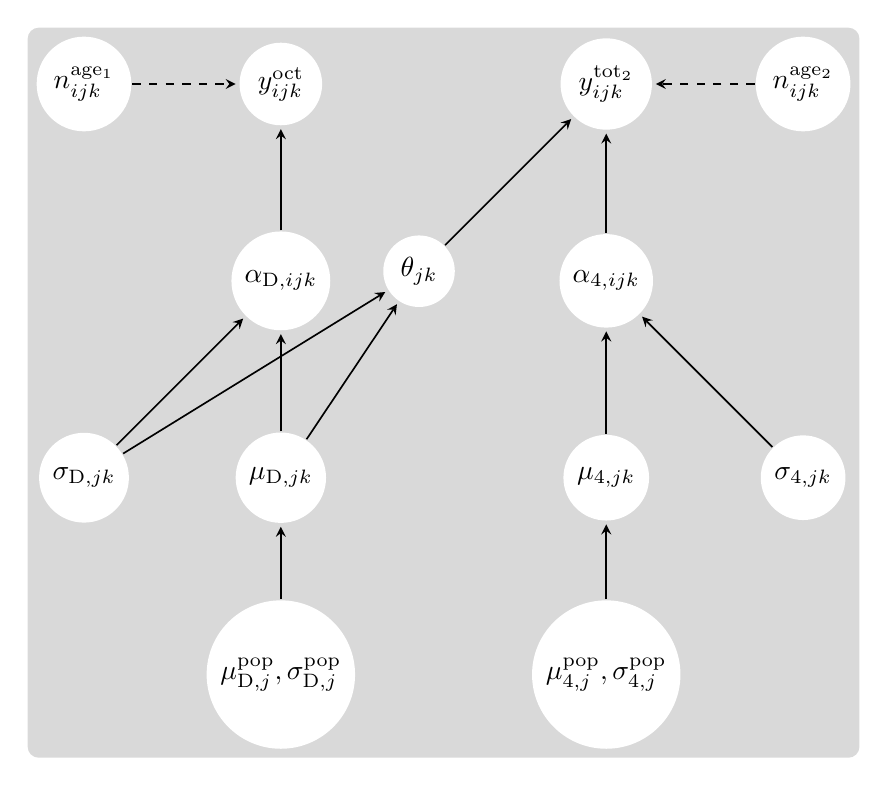
\begin{tikzpicture}[
            > = stealth, % arrow head style
            shorten > = 1pt, % don't touch arrow head to node
            auto,
            node distance = 2.5cm, % distance between nodes
            semithick % line style
            ]

        \tikzstyle{every state}=[
            draw = none,
            thick,
            fill = white,
            minimum size = 4mm
        ]F


	% data level
        \node[state] (N2) [] {$n^\mathrm{age_1}_{ijk}$};
	\node[state] (Y2) [right of=N2] {$y^{\mathrm{oct}}_{ijk}$};
       
        \path[dashed,->] (N2) edge node {} (Y2);
	
        \node[state] (Y) [right = 3cm of Y2] {$y^{\mathrm{tot_2}}_{ijk}$};
        \node[state] (N) [right of=Y] {$n^\mathrm{age_2}_{ijk}$};
       
        \path[dashed,->] (N) edge node {} (Y);
        


	% link models
	 \node[state] (AB3) [below left  =2.3cm of Y] {$\theta_{jk}$};  


        % probability
        % \node[state] (T) [below of = Y] {$\theta_{ijk}$};
        %       
        % \path[->] (T) edge node {} (Y);
                  
        % hyperparameters
         \node[state] (AB) [below of = Y] {$\alpha_{4,ijk}$};  
         \path[->] (AB) edge node {} (Y);
         
         \node[state] (AB2) [below of = Y2] {$\alpha_{\mathrm{D},ijk}$};
         \path[->] (AB2) edge node {} (Y2);
               
          % hyperparameters
        
         \node[state] (MS) [below of = AB] {$\mu_{4,jk}$};
         \node[state] (A) [right of = MS] {$\sigma_{4,jk}$};
         
         \path[->] (A) edge node {} (AB);       
         \path[->] (MS) edge node {} (AB);       
         
         \node[state] (H) [below of = MS] {$\mu^\mathrm{pop}_{4,j},\sigma^\mathrm{pop}_{4,j}$};
         \path[->] (H) edge node {} (MS);       
         
         \node[state] (MS2) [below of = AB2] {$\mu_{\mathrm{D},jk}$};
         \node[state] (A2) [left of = MS2] {$\sigma_{\mathrm{D},jk}$};
         
         \path[->] (A2) edge node {} (AB2);       
         \path[->] (MS2) edge node {} (AB2);       
         
         \node[state] (H2) [below of = MS2] {$\mu^\mathrm{pop}_{\mathrm{D},j},\sigma^\mathrm{pop}_{\mathrm{D},j}$};
         \path[->] (H2) edge node {} (MS2);       

% link nodes
         \path[->] (AB3) edge node {} (Y);
         \path[->] (A2) edge node {} (AB3);       
         \path[->] (MS2) edge node {} (AB3);       
         
          \begin{scope}[on background layer]
   \node [fit=(N2) (N) (H2), fill= gray!30, rounded corners, inner sep=.1cm] {};
  \end{scope}
         
  \end{tikzpicture}
  %
    \hspace{1cm}% NO SPACE!
  % BEGIN FIGURE 3
   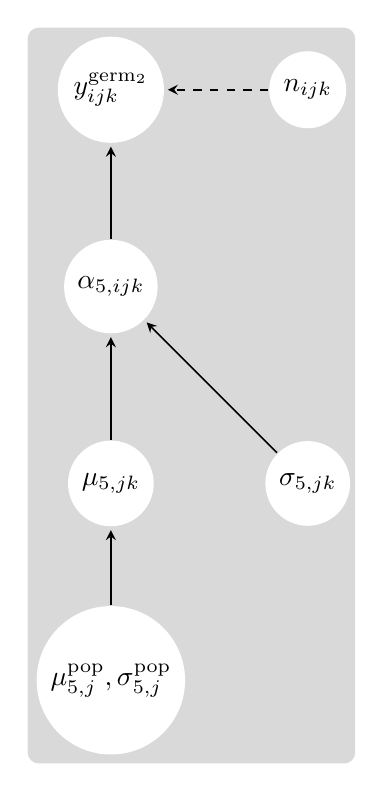
\begin{tikzpicture}[
            > = stealth, % arrow head style
            shorten > = 1pt, % don't touch arrow head to node
            auto,
            node distance = 2.5cm, % distance between nodes
            semithick % line style
        ]

        \tikzstyle{every state}=[
            draw = none,
            thick,
            fill = white,
            minimum size = 4mm
        ]F


	% data level
        \node[state] (Y) [] {$y^{\mathrm{germ_2}}_{ijk}$};
        \node[state] (N) [right of=Y] {$n_{ijk}$};
       
        \path[dashed,->] (N) edge node {} (Y);

        % probability
        % \node[state] (T) [below of = Y] {$\theta_{ijk}$};
        %       
        % \path[->] (T) edge node {} (Y);
                  
                  % hyperparameters
         \node[state] (AB) [below of = Y] {$\alpha_{5,ijk}$};
                
         \path[->] (AB) edge node {} (Y);
         
          % hyperparameters
        
         \node[state] (MS) [below of = AB] {$\mu_{5,jk}$};
         \node[state] (A) [right of = MS] {$\sigma_{5,jk}$};
         
         \path[->] (A) edge node {} (AB);       
         \path[->] (MS) edge node {} (AB);       
         
         \node[state] (H) [below of = MS] {$\mu^\mathrm{pop}_{5,j},\sigma^\mathrm{pop}_{5,j}$};
         \path[->] (H) edge node {} (MS);       
         
   \begin{scope}[on background layer]
   \node [fit=(Y) (N) (H), fill= gray!30, rounded corners, inner sep=.1cm] {};
  \end{scope}
                                 
  \end{tikzpicture}
\subcaption{Directed acyclic graphs for the hierarchical models for seed bag rates (age 2). Solid arrows depict the relationships among random variables, and dashed arrows depict the deterministic relationships.}
\end{subfigure}
\end{figure}


%%%%%%%%%%%%%%%%%%%%%%%%%%%%%%%%%%%%%%%%%%%%%%%%%%%%
% POSTERIOR AND JOINT DISTRIBUTIONS FOR AGE 2 SEED BAGS
%%%%%%%%%%%%%%%%%%%%%%%%%%%%%%%%%%%%%%%%%%%%%%%%%%%%

% QUESTIONS
% do I need to include \bm{n} on the RHS of the conditional statement for the posterior?

\begin{align}
  \begin{split}
  [  \bm{\alpha_\mathrm{D}} , &  \bm{\alpha_4}, \bm{\theta}, \bm{\mu_\mathrm{D}} , \bm{\sigma_\mathrm{D}} , \bm{\mu_4} , \bm{\sigma_4} , \bm{\mu^\mathrm{pop}_\mathrm{D}}, \bm{\sigma^\mathrm{pop}_\mathrm{D}} , \bm{\mu^\mathrm{pop}_4}, \bm{\sigma^\mathrm{pop}_4} | \bm{y^\mathrm{oct}} , \bm{y^\mathrm{tot_2}}  ]  \propto  \\  
 	     & \prod_{j=1}^{J} \bigg\{ \Big\{ \prod_{i=1}^{N_1}  \prod_{k=1}^{K_1} \mathrm{binomial} \big( y^{\mathrm{oct}}_{ijk} | n^\mathrm{age_1}_{ijk}, \mathrm{logit}^{-1}( \alpha_{\mathrm{D},ijk} ) \big) \\
	      \times & \mathrm{normal} ( \alpha_{\mathrm{D},ijk}  | \mu_{\mathrm{D},jk}, \sigma{_{\mathrm{D},jk} }) \mathrm{normal} ( \mu_{\mathrm{D},jk}  | \mu^\mathrm{pop}_{\mathrm{D},j}, \sigma^\mathrm{pop}_{\mathrm{D},j} ) 
 \textrm{half-normal} ( \sigma_{\mathrm{D},jk} | 0,1) \\
 \times & \mathrm{normal} ( \mu^\mathrm{pop}_{\mathrm{D},j} | 0 , 1000 ) \textrm{half-normal} ( \sigma^\mathrm{pop}_{\mathrm{D},j} | 0,1)   \Big\}  \\
  \times &  \Big\{ \prod_{i=1}^{N_2}  \prod_{k=1}^{K_2}   \mathrm{binomial} \big( y^{\mathrm{tot_2}}_{ijk} | n^\mathrm{age_2}_{ijk}, \mathrm{logit}^{-1}( \alpha_{\mathrm{4},ijk} ) \times \theta_{jk} \big) \\
   \times & \mathrm{normal} ( \theta_{jk}  | \mu_{\mathrm{D},jk}, \sigma{_{\mathrm{D},jk} }) \\
    \times & \mathrm{normal} ( \alpha_{\mathrm{4},ijk}  | \mu_{\mathrm{4},jk}, \sigma{_{\mathrm{4},jk} }) \mathrm{normal} ( \mu_{\mathrm{4},jk}  | \mu^\mathrm{pop}_{\mathrm{4},j}, \sigma^\mathrm{pop}_{\mathrm{4},j} ) \textrm{half-normal} ( \sigma_{\mathrm{4},jk} | 0,1) \\
    \times & \mathrm{normal} ( \mu^\mathrm{pop}_{\mathrm{4},j} | 0 , 1000 ) \textrm{half-normal} ( \sigma^\mathrm{pop}_{\mathrm{4},j} | 0,1) \Big\}  \bigg\}.
  \end{split}
\end{align}


%
\begin{align}
  \begin{split}
 [  \bm{\alpha_5} , \bm{\mu_5} , \bm{\sigma_5} , \bm{\mu^\mathrm{pop}_5}, \bm{\sigma^\mathrm{pop}_5} | & \bm{y^{\mathrm{total}}}  ] \propto \prod_{i=1}^{I}   \prod_{j=1}^{J}  \prod_{k=1}^{K} 
   \mathrm{binomial} ( y^{\mathrm{tot}}_{ijk} | n^\mathrm{tot}_{ijk}, \mathrm{logit}^{-1}( \alpha_{5,ijk} ) ) 
   \\ & \times \mathrm{normal} ( \alpha_{5,ijk}  | \mu_{5,jk}, \sigma{_{5,jk} })
  \\ & \times \mathrm{normal} ( \mu_{5,jk}  | \mu^\mathrm{pop}_{5,j}, \sigma^\mathrm{pop}_{5,j} )
  \\ & \times \textrm{half-normal} ( \sigma_{5,jk} | 0,1)
  \\ & \times \mathrm{normal} ( \mu^\mathrm{pop}_{5,j} | 0 , 1000 ) \textrm{half-normal} ( \sigma^\mathrm{pop}_{5,j} | 0,1).
  \end{split}
\end{align}

\clearpage
\newpage


\subsection*{Viability trials}

%%%%%%%%%%%%%%%%%%%%%%%%%%%%%%%%%%%%%%%%%%%%%%%%%%%%
% DIRECTED ACYCLIC GRAPHS FOR VIABILITY TRIALS
%%%%%%%%%%%%%%%%%%%%%%%%%%%%%%%%%%%%%%%%%%%%%%%%%%%%
\begin{figure}[h]%
\begin{subfigure}[c]{\textwidth}
\centering
   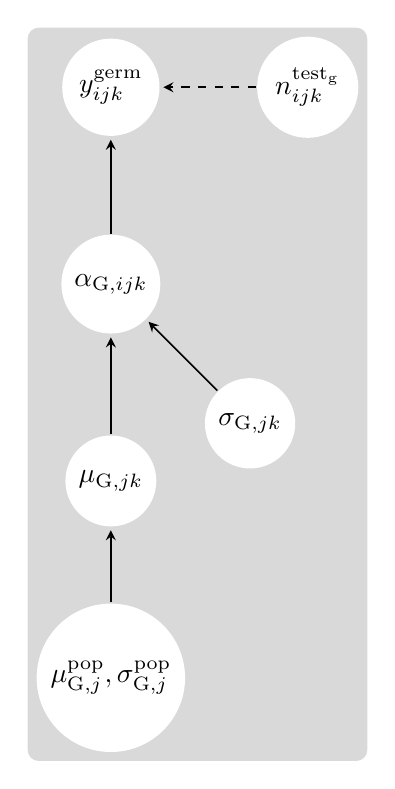
\begin{tikzpicture}[
            > = stealth, % arrow head style
            shorten > = 1pt, % don't touch arrow head to node
            auto,
            node distance = 2.5cm, % distance between nodes
            semithick % line style
        ]

        \tikzstyle{every state}=[
            draw = none,
            thick,
            fill = white,
            minimum size = 4mm
        ]F


	% data level
        \node[state] (Y) [] {$y^{\mathrm{germ}}_{ijk}$};
        \node[state] (N) [right of=Y] {$n^\mathrm{test_g}_{ijk}$};
       
        \path[dashed,->] (N) edge node {} (Y);

        % probability
        % \node[state] (T) [below of = Y] {$\theta_{ijk}$};
        %       
        % \path[->] (T) edge node {} (Y);
                  
                  % hyperparameters
         \node[state] (AB) [below of = Y] {$\alpha_{\mathrm{G},ijk}$};
                
         \path[->] (AB) edge node {} (Y);
         
          % hyperparameters
        
         \node[state] (MS) [below of = AB] {$\mu_{\mathrm{G},jk}$};
         \node[state] (A) [below right of = AB] {$\sigma_{\mathrm{G},jk}$};
         
         \path[->] (A) edge node {} (AB);       
         \path[->] (MS) edge node {} (AB);       
         
         \node[state] (H) [below of = MS] {$\mu^\mathrm{pop}_{\mathrm{G},j},\sigma^\mathrm{pop}_{\mathrm{G},j}$};
         \path[->] (H) edge node {} (MS);       

                    \begin{scope}[on background layer]
   \node [fit=(Y) (N) (H), fill= gray!30, rounded corners, inner sep=.1cm] {};
  \end{scope}
  
  \end{tikzpicture}
  %
    \hspace{1cm}% NO SPACE!
  % BEGIN FIGURE 3
   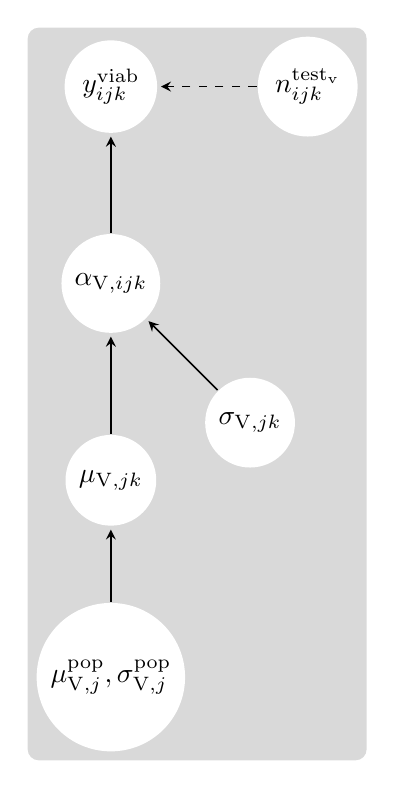
\begin{tikzpicture}[
            > = stealth, % arrow head style
            shorten > = 1pt, % don't touch arrow head to node
            auto,
            node distance = 2.5cm, % distance between nodes
            semithick % line style
        ]

        \tikzstyle{every state}=[
            draw = none,
            thick,
            fill = white,
            minimum size = 4mm
        ]F


	% data level
        \node[state] (Y) [] {$y^{\mathrm{viab}}_{ijk}$};
        \node[state] (N) [right of=Y] {$n^\mathrm{test_v}_{ijk}$};
       
        \path[dashed,->] (N) edge node {} (Y);

        % probability
        % \node[state] (T) [below of = Y] {$\theta_{ijk}$};
        %       
        % \path[->] (T) edge node {} (Y);
                  
                  % hyperparameters
         \node[state] (AB) [below of = Y] {$\alpha_{\mathrm{V},ijk}$};
                
         \path[->] (AB) edge node {} (Y);
         
          % hyperparameters
        
         \node[state] (MS) [below of = AB] {$\mu_{\mathrm{V},jk}$};
         \node[state] (A) [below right of = AB] {$\sigma_{\mathrm{V},jk}$};
         
         \path[->] (A) edge node {} (AB);       
         \path[->] (MS) edge node {} (AB);       
         
         \node[state] (H) [below of = MS] {$\mu^\mathrm{pop}_{\mathrm{V},j},\sigma^\mathrm{pop}_{\mathrm{V},j}$};
         \path[->] (H) edge node {} (MS);      
         
                             \begin{scope}[on background layer]
   \node [fit=(Y) (N) (H), fill= gray!30, rounded corners, inner sep=.1cm] {};
  \end{scope}
                                
  \end{tikzpicture}
\subcaption{Directed acyclic graphs for the hierarchical models for viability trials. Solid arrows depict the relationships among random variables, and dashed arrows depict the deterministic relationships.}
\end{subfigure}
\end{figure}
%
%%%%%%%%%%%%%%%%%%%%%%%%%%%%%%%%%%%%%%%%%%%%%%%%%%%%
% POSTERIOR AND JOINT DISTRIBUTIONS FOR VIABILITY TRIALS
%%%%%%%%%%%%%%%%%%%%%%%%%%%%%%%%%%%%%%%%%%%%%%%%%%%%

% QUESTIONS
% do I need to include \bm{n} on the RHS of the conditional statement for the posterior?

\begin{align}
  \begin{split}
 [  \bm{\alpha_G} , \bm{\mu_G} , \bm{\sigma_G} , \bm{\mu^\mathrm{pop}_G}, \bm{\sigma^\mathrm{pop}_G} | & \bm{y^{\mathrm{tot}}}  ] \propto \prod_{i=1}^{I}   \prod_{j=1}^{J}  \prod_{k=1}^{K} 
   \mathrm{binomial} ( y^{\mathrm{germ}}_{ijk} | n^\mathrm{test_g}_{ijk}, \mathrm{logit}^{-1}( \alpha_{G,ijk} ) ) 
   \\ & \times \mathrm{normal} ( \alpha_{G,ijk}  | \mu_{G,jk}, \sigma{_{G,jk} })
  \\ & \times \mathrm{normal} ( \mu_{G,jk}  | \mu^\mathrm{pop}_{G,j}, \sigma^\mathrm{pop}_{G,j} )
  \\ & \times \textrm{half-normal} ( \sigma_{G,jk} | 0,1)
  \\ & \times \mathrm{normal} ( \mu^\mathrm{pop}_{G,j} | 0 , 1000 ) \textrm{half-normal} ( \sigma^\mathrm{pop}_{G,j} | 0,1).
  \end{split}
\end{align}
%
\begin{align}
  \begin{split}
 [  \bm{\alpha_V} , \bm{\mu_V} , \bm{\sigma_V} , \bm{\mu^\mathrm{pop}_V}, \bm{\sigma^\mathrm{pop}_V} | & \bm{y^{\mathrm{tot}}}  ] \propto \prod_{i=1}^{I}   \prod_{j=1}^{J}  \prod_{k=1}^{K} 
   \mathrm{binomial} ( y^{\mathrm{viab}}_{ijk} | n^\mathrm{test_v}_{ijk}, \mathrm{logit}^{-1}( \alpha_{V,ijk} ) ) 
   \\ & \times \mathrm{normal} ( \alpha_{V,ijk}  | \mu_{V,jk}, \sigma{_{V,jk} })
  \\ & \times \mathrm{normal} ( \mu_{V,jk}  | \mu^\mathrm{pop}_{V,j}, \sigma^\mathrm{pop}_{V,j} )
  \\ & \times \textrm{half-normal} ( \sigma_{V,jk} | 0,1)
  \\ & \times \mathrm{normal} ( \mu^\mathrm{pop}_{V,j} | 0 , 1000 ) \textrm{half-normal} ( \sigma^\mathrm{pop}_{V,j} | 0,1).
  \end{split}
\end{align}
%

\clearpage
\newpage

\subsection*{Survival of seedlings to fruiting plants}

%%%%%%%%%%%%%%%%%%%%%%%%%%%%%%%%%%%%%%%%%%%%%%%%%%%%
% DIRECTED ACYCLIC GRAPHS FOR SEED SURVIVAL
%%%%%%%%%%%%%%%%%%%%%%%%%%%%%%%%%%%%%%%%%%%%%%%%%%%%
\begin{figure}[!h]%
\begin{subfigure}[c]{\textwidth}
\centering
   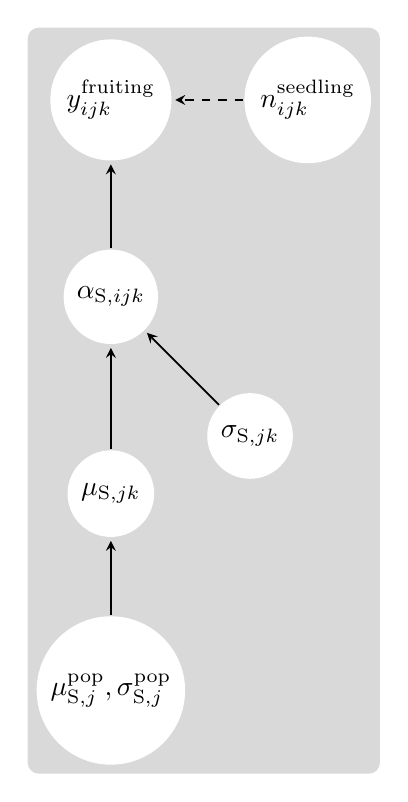
\begin{tikzpicture}[
            > = stealth, % arrow head style
            shorten > = 1pt, % don't touch arrow head to node
            auto,
            node distance = 2.5cm, % distance between nodes
            semithick % line style
        ]

        \tikzstyle{every state}=[
            draw = none,
            thick,
            fill = white,
            minimum size = 4mm
        ]F
% data level
        \node[state] (Y) [] {$y^{\mathrm{fruiting}}_{ijk}$};
        \node[state] (N) [right of=Y] {$n^\mathrm{seedling}_{ijk}$};
       
        \path[dashed,->] (N) edge node {} (Y);

        % probability
        % \node[state] (T) [below of = Y] {$\theta_{ijk}$};
        %       
        % \path[->] (T) edge node {} (Y);
                  
                  % hyperparameters
         \node[state] (AB) [below of = Y] {$\alpha_{\mathrm{S},ijk}$};
                
         \path[->] (AB) edge node {} (Y);
         
          % hyperparameters
        
         \node[state] (MS) [below of = AB] {$\mu_{\mathrm{S},jk}$};
         \node[state] (A) [below right of = AB] {$\sigma_{\mathrm{S},jk}$};
         
         \path[->] (A) edge node {} (AB);       
         \path[->] (MS) edge node {} (AB);       
         
         \node[state] (H) [below of = MS] {$\mu^\mathrm{pop}_{\mathrm{S},j},\sigma^\mathrm{pop}_{\mathrm{S},j}$};
         \path[->] (H) edge node {} (MS);       

                    \begin{scope}[on background layer]
   \node [fit=(Y) (N) (H), fill= gray!30, rounded corners, inner sep=.1cm] {};
  \end{scope}
  
  \end{tikzpicture}

\subcaption{Directed acyclic graphs for the hierarchical models for seed survival. Solid arrows depict the relationships among random variables, and dashed arrows depict the deterministic relationships.}
\end{subfigure}
\end{figure}

%
%%%%%%%%%%%%%%%%%%%%%%%%%%%%%%%%%%%%%%%%%%%%%%%%%%%%
% POSTERIOR AND JOINT DISTRIBUTIONS FOR SEED SURVIVAL
%%%%%%%%%%%%%%%%%%%%%%%%%%%%%%%%%%%%%%%%%%%%%%%%%%%%

% QUESTIONS
% do I need to include \bm{n} on the RHS of the conditional statement for the posterior?

\begin{align}
  \begin{split}
 [  \bm{\alpha_S} , \bm{\mu_S} , \bm{\sigma_S} , \bm{\mu^\mathrm{pop}_S}, \bm{\sigma^\mathrm{pop}_S} | & \bm{y^{\mathrm{fruiting}}}  ] \propto \prod_{i=1}^{I}   \prod_{j=1}^{J}  \prod_{k=1}^{K} 
   \mathrm{binomial} ( y^{\mathrm{fruiting}}_{ijk} | n^\mathrm{seedling}_{ijk}, \mathrm{logit}^{-1}( \alpha_{S,ijk} ) ) 
   \\ & \times \mathrm{normal} ( \alpha_{S,ijk}  | \mu_{S,jk}, \sigma{_{S,jk} })
  \\ & \times \mathrm{normal} ( \mu_{S,jk}  | \mu^\mathrm{pop}_{S,j}, \sigma^\mathrm{pop}_{S,j} )
  \\ & \times \textrm{half-normal} ( \sigma_{S,jk} | 0,1)
  \\ & \times \mathrm{normal} ( \mu^\mathrm{pop}_{S,j} | 0 , 1000 ) \textrm{half-normal} ( \sigma^\mathrm{pop}_{S,j} | 0,1).
  \end{split}
\end{align}


\clearpage
\newpage

\subsection*{Fruits per plant and seeds per fruit}

%%%%%%%%%%%%%%%%%%%%%%%%%%%%%%%%%%%%%%%%%%%%%%%%%%%%
% DIRECTED ACYCLIC GRAPHS FOR FECUNDITY
%%%%%%%%%%%%%%%%%%%%%%%%%%%%%%%%%%%%%%%%%%%%%%%%%%%%
\begin{figure}[h]%
\begin{subfigure}[c]{\textwidth}
\centering
   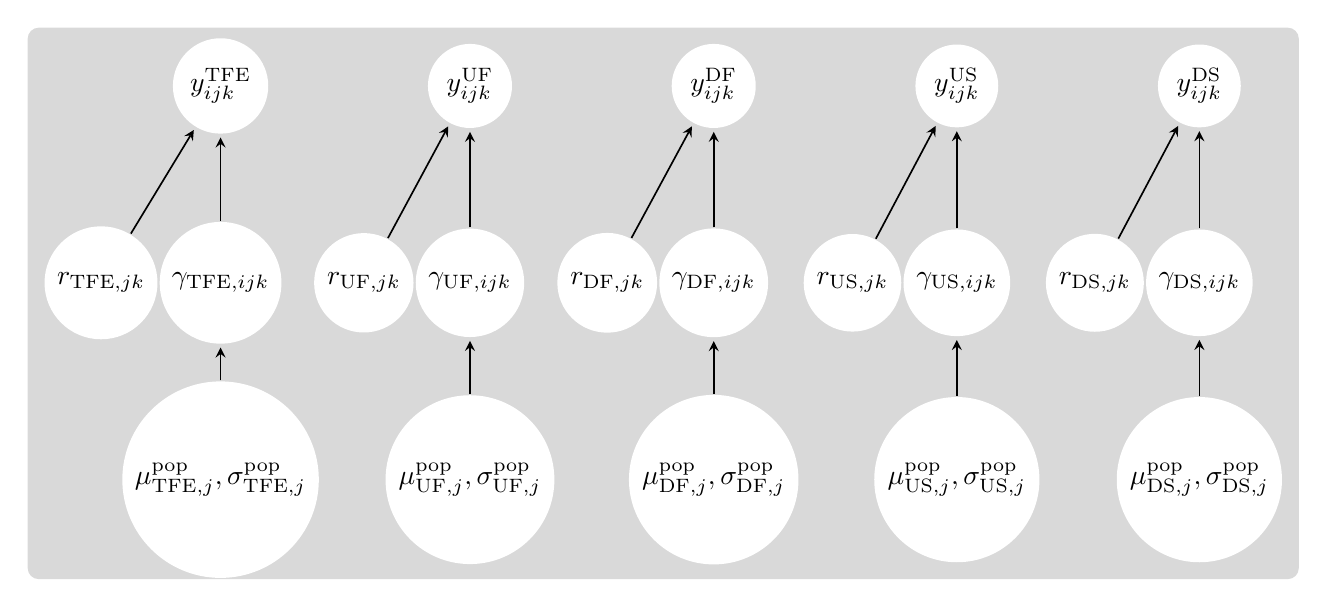
\begin{tikzpicture}[
            > = stealth, % arrow head style
            shorten > = 1pt, % don't touch arrow head to node
            auto,
            node distance = 2.5cm, % distance between nodes
            semithick % line style
            ]

        \tikzstyle{every state}=[
            draw = none,
            thick,
            fill = white,
            minimum size = 4mm
        ]F


	% data level
	\node[state] (Y) [] {$y^{\mathrm{UF}}_{ijk}$};
	\node[state] (Y2) [left =2cm of Y] {$y^{\mathrm{TFE}}_{ijk}$};
       	\node[state] (Y3) [right  =2cm of Y] {$y^{\mathrm{DF}}_{ijk}$};
         \node[state] (Y4) [right  =2cm of Y3] {$y^{\mathrm{US}}_{ijk}$};
         \node[state] (Y5) [right  =2cm of Y4] {$y^{\mathrm{DS}}_{ijk}$};
    
        
        % rparameters
         \node[state] (A) [below of = Y] {$\gamma_{\mathrm{UF},ijk}$};  
         \path[->] (A) edge node {} (Y);
         \node[state] (B) [left = 0cm of A] {$r_{\mathrm{UF},jk}$};  
         \path[->] (B) edge node {} (Y);
               
         \node[state] (A2) [below of = Y2] {$\gamma_{\mathrm{TFE},ijk}$};
         \path[->] (A2) edge node {} (Y2);
         \node[state] (B2) [left = 0cm of A2] {$r_{\mathrm{TFE},jk}$};  
         \path[->] (B2) edge node {} (Y2);
                  
         \node[state] (A3) [below of = Y3] {$\gamma_{\mathrm{DF},ijk}$};
         \path[->] (A3) edge node {} (Y3);
         \node[state] (B3) [left = 0cm of A3] {$r_{\mathrm{DF},jk}$};  
         \path[->] (B3) edge node {} (Y3);
                  
                  \node[state] (A4) [below of = Y4] {$\gamma_{\mathrm{US},ijk}$};
         \path[->] (A4) edge node {} (Y4);
         \node[state] (B4) [left = 0cm of A4] {$r_{\mathrm{US},jk}$};  
         \path[->] (B4) edge node {} (Y4);
          
                   \node[state] (A5) [below of = Y5] {$\gamma_{\mathrm{DS},ijk}$};
         \path[->] (A5) edge node {} (Y5);           
         \node[state] (B5) [left = 0cm of A5] {$r_{\mathrm{DS},jk}$};  
         \path[->] (B5) edge node {} (Y5);
                     
          % hyperparameters
         \node[state] (C) [below of = A] {$\mu^\mathrm{pop}_{\mathrm{UF},j},\sigma^\mathrm{pop}_{\mathrm{UF},j}$};
         \path[->] (C) edge node {} (A);           
         
                  \node[state] (C2) [below of = A2] {$\mu^\mathrm{pop}_{\mathrm{TFE},j},\sigma^\mathrm{pop}_{\mathrm{TFE},j}$};
         \path[->] (C2) edge node {} (A2);         
         
                  \node[state] (C3) [below of = A3] {$\mu^\mathrm{pop}_{\mathrm{DF},j},\sigma^\mathrm{pop}_{\mathrm{DF},j}$};
         \path[->] (C3) edge node {} (A3);         
         
          \node[state] (C4) [below of = A4] {$\mu^\mathrm{pop}_{\mathrm{US},j},\sigma^\mathrm{pop}_{\mathrm{US},j}$};
         \path[->] (C4) edge node {} (A4);      

          \node[state] (C5) [below of = A5] {$\mu^\mathrm{pop}_{\mathrm{DS},j},\sigma^\mathrm{pop}_{\mathrm{DS},j}$};
         \path[->] (C5) edge node {} (A5);      
                                  
          \begin{scope}[on background layer]
   \node [fit=(B2) (Y5) (C5), fill= gray!30, rounded corners, inner sep=.2cm] {};
  \end{scope}
                                 
  \end{tikzpicture}
\subcaption{Directed acyclic graphs for the hierarchical models fruits per plant and seeds per fruit. Solid arrows depict the relationships among random variables, and dashed arrows depict the deterministic relationships.}
\end{subfigure}
\end{figure}

%
%%%%%%%%%%%%%%%%%%%%%%%%%%%%%%%%%%%%%%%%%%%%%%%%%%%%
% POSTERIOR AND JOINT DISTRIBUTIONS FOR FECUNDITY
%%%%%%%%%%%%%%%%%%%%%%%%%%%%%%%%%%%%%%%%%%%%%%%%%%%%

% QUESTIONS
% do I need to include \bm{n} on the RHS of the conditional statement for the posterior?

\begin{align}
  \begin{split}
  [  \bm{\alpha_\mathrm{D}} , &  \bm{\alpha_4}, \bm{\theta}, \bm{\mu_\mathrm{D}} , \bm{\sigma_\mathrm{D}} , \bm{\mu_4} , \bm{\sigma_4} , \bm{\mu^\mathrm{pop}_\mathrm{D}}, \bm{\sigma^\mathrm{pop}_\mathrm{D}} , \bm{\mu^\mathrm{pop}_4}, \bm{\sigma^\mathrm{pop}_4} | \bm{y^\mathrm{oct}} , \bm{y^\mathrm{tot_2}}  ]  \propto  \\  
 	     & \prod_{j=1}^{J} \bigg\{ \Big\{ \prod_{i=1}^{N_1}  \prod_{k=1}^{K_1} \mathrm{binomial} \big( y^{\mathrm{oct}}_{ijk} | n^\mathrm{age_1}_{ijk}, \mathrm{logit}^{-1}( \alpha_{\mathrm{D},ijk} ) \big) \\
	      \times & \mathrm{normal} ( \alpha_{\mathrm{D},ijk}  | \mu_{\mathrm{D},jk}, \sigma{_{\mathrm{D},jk} }) \mathrm{normal} ( \mu_{\mathrm{D},jk}  | \mu^\mathrm{pop}_{\mathrm{D},j}, \sigma^\mathrm{pop}_{\mathrm{D},j} ) 
 \textrm{half-normal} ( \sigma_{\mathrm{D},jk} | 0,1) \\
 \times & \mathrm{normal} ( \mu^\mathrm{pop}_{\mathrm{D},j} | 0 , 1000 ) \textrm{half-normal} ( \sigma^\mathrm{pop}_{\mathrm{D},j} | 0,1)   \Big\}  \\
  \times &  \Big\{ \prod_{i=1}^{N_2}  \prod_{k=1}^{K_2}   \mathrm{binomial} \big( y^{\mathrm{tot_2}}_{ijk} | n^\mathrm{age_2}_{ijk}, \mathrm{logit}^{-1}( \alpha_{\mathrm{4},ijk} ) \times \theta_{jk} \big) \\
   \times & \mathrm{normal} ( \theta_{jk}  | \mu_{\mathrm{D},jk}, \sigma{_{\mathrm{D},jk} }) \\
    \times & \mathrm{normal} ( \alpha_{\mathrm{4},ijk}  | \mu_{\mathrm{4},jk}, \sigma{_{\mathrm{4},jk} }) \mathrm{normal} ( \mu_{\mathrm{4},jk}  | \mu^\mathrm{pop}_{\mathrm{4},j}, \sigma^\mathrm{pop}_{\mathrm{4},j} ) \textrm{half-normal} ( \sigma_{\mathrm{4},jk} | 0,1) \\
    \times & \mathrm{normal} ( \mu^\mathrm{pop}_{\mathrm{4},j} | 0 , 1000 ) \textrm{half-normal} ( \sigma^\mathrm{pop}_{\mathrm{4},j} | 0,1) \Big\}  \bigg\}.
  \end{split}
\end{align}


\end{document}
